\newcommand\showchange{FL}%{TT FL}%
\documentclass[preprint,10pt]{sigplanconf}
\usepackage{times}
\usepackage{graphicx}
\usepackage{tabularx}
\usepackage{subfigure}
\usepackage{color}
\usepackage{xcolor}
%\usepackage{caption}
%\usepackage{subcaption}
\usepackage{multirow}
%\usepackage{cite}	% sort citation numbers
\usepackage{url}
\usepackage{xspace}
%\usepackage[compact]{titlesec}
%\usepackage{amsmath}


%%%%%%%%%%%%%%%%%%%%%%
% Select one or other if want to see comments.
% \com is sometimes displayed during draft.
\long\def\com#1{}
%\long\def\com#1{{\bf \sc comment: }{\small [#1]}{\bf \sc\ endcomment}\newline}

\long\def\xxx#1{{\bf XXX: }{\small [#1]}}
%\long\def\xxx#1{}

%\if\showchange
%\usepackage[usenames,dvipsnames]{color}
%\newcommand\bluet[1]{\color{blue}{#1}}
%\newcommand\redt[1]{\textcolor{red}{#1}}
%\else
%\newcommand\bluet[1]{#1}
%\newcommand\redt[1]{#1}
%\fi

% Use this macro to force page breaks where ugly widows/orphans occur;
% be sure to recheck all uses after any significant change to the text!
\def\widowpage{\pagebreak}

% Choose abbreviated or long-version alternatives in paper
\long\def\abbr#1#2{#1}			% abbreviated version
%\long\def\abbr#1#2{#2}			% long version

% Choose abbreviations or long names/titles in bibliography
\def\bibbrev#1#2{#1}			% short version
%\def\bibbrev#1#2{#2}			% long version
%\def\bibbrev#1#2{\abbr{#1}{#2}}		% follow abbr macro

% Abbreviated or full citation lists: \abcite{basic}{others}
\newcommand{\abcite}[2]{\abbr{\cite{#1}}{\cite{#1,#2}}}

% Conference abbreviations: \bibconf[Nth]{SOSP}{Symposium on ...}
\newcommand{\bibconf}[3][]{#1 \bibbrev{#2}{#3 (#2)}}

% Stuff to eliminate for blind review
%\newcommand{\blind}[1]{#1}		% non-blind
\newcommand{\blind}[1]{}		% blind
%%%%%%%%%%%%%%%%%%%%%%

\newcommand{\kn}[1]{\texttt{\small #1}} % key name
\newcommand{\kw}[1]{{\em #1}}        	% keyword
%\newcommand\code[1]{{\scriptsize \textsf{#1}}}
\newcommand\codet[1]{{\small \textsf{#1}}}
\newcommand\code[1]{{\small \textit{#1}}}
\newcommand\ie{{\em i.e.,}\xspace}             % i.e.
\newcommand\eg{{e.g.,}\xspace}             	% e.g.
\newcommand\myds{{\bf\em{SMR}}\xspace}
\newcommand\myth{{\bf\em{Sthread}}\xspace}
\newcommand\mydsname{({\bf\em s}calable {\bf\em u}nbounded {\bf\em m}ulticast {\bf\em C}hannel)\xspace}
\newcommand\Oflag{{\tt O}\xspace}
\newcommand\Pflag{{\tt P}\xspace}
\newcommand\Wflag{{\tt W}\xspace}

\newcommand{\grayt}[1]{{\color{gray} #1}}
\newcommand{\redt}[1]{{\color{red} #1}}
\newcommand{\bluet}[1]{{\color{blue} #1}}




\title{\vspace{-5pt} SMR: A good scalability MapReduce for Multicore Systems\\
  
	\vspace{-5pt}}
\authorinfo{}{}{}
\iffalse
\authorinfo{# \and }
	{University of Science and Technology of China}
	{yufeny@ustc.mail.edu.cn}
\fi
\iffalse
\conferenceinfo{'11,} {July 11-12, 2011, Shanghai, China.}
\CopyrightYear{2011}
\crdata{978-1-4503-1179-3/11/07}
\clubpenalty=10000
\widowpenalty=10000
\fi
\begin{document}

\maketitle

\begin{abstract}
Designing and implementing efficient, simply
parallel programming model is challenging.
Traditional parallel programming techniques
like Pthreads and OpenMPI leave programmers
solving many details of design chanllenges.
Dynamic runtimes can simplify parallel programming 
by automatically managing concurrency without
further burdening the programmer. 
Nevertheless, implementing such runtime systems for large-scale, shared-memory systems
can be challenging.
Phoenix, a MapReduce library for multicore, 
show that MapReduce is a promising model 
for scalable performance on mulitcore and multiprocess.
Applications written with MapReduce framwork
have competitive scalability and performance
comparied to those written with Pthreads.


%Our previous work, DMR\cite{zhang2015dmr}, a deterministic MapReduce for multicore,
%is a safe and efficient alternative to Phoenix. 
%In addition, evaluation results show 
%application like \textit{pca} and \textit{word\_count} have better 
%scalabiliy and performans than Phoenix. 

This work presents \myds, a modified version of phoenix framwork 
(...)
We evaluated \myds on a 32 CPU cores process.
The results show that \myds achieves up to (NUM1) speedup over Phoenix.
\end{abstract}

%\input{terms}
\section{Introduction}
\label{sec:intro}

%%需要调研的部分:解答的问题,为什么我们关注多核的scalability问题。随着分布式系统的广泛普及,企业和用户的通用的做法是通过堆积更多的机器来获取更快的处理效率和速度。但是机器堆积的越多,网络带宽,耗电也越来越多,如何充分利用单台机器的多核资源成为很重要的课题。

%一方面,随着多核机器的广泛普及,如何充分利用多核资源成为非常重要的课题,另一方面,现有的很多我们希望充分利用单台机器上的资源,

%目前的现状,需求
As the prevalence of multicore chips,
it is foreseeable that tens to hundreds (even thousands) of cores on a single chip
will appear in the near future\cite{Borkar2007core}.
While utilizing multicore sources is still challenging
because of the difficulties of parallel programming.
Specifically, the thread-based model requires the programmer to manually
manage synchronization, load balancing, and locality, which is
often error-prone (e.g., races and deadlocks) or requires detailed
understanding of the underlying hardware.
An alternative approach is to rely on a runtime system for
concurrency management. 

MapReduce\cite{dean2004mapreduce}, 
for instance, is a promising programming model for clusters
to perform large-scale data processing
in a simple and efficient way.
In most cases, programmers only need to implement two functions:
map and reduce.
The runtime system spawns multiple threads that apply
these functions concurrently across the elements of the input
dataset. 
%The runtime spawns multiple threads to worker and 
%automatically manages synchronization, load balancing, 
%and locality in order to achieve efficient execution.
%which aggregates values in the key-value pairs according to the key.
And the programmer dose no need to control synchronization 
and schedule tasks manually.
%面向多核的MapReduce的相关工作
While initially MapReduce is implemented on clusters, Ranger
et al. have demonstrated the feasibility of running MapReduce
applications on shared memory multicore machines with 
Phoenix\cite{ranger2007phoenix}.
Other libraries such as Metis\cite{mao2010metis} 
, Tiled-mapreduce\cite{chen2010tiled} and MRPhi\cite{lu2013mrphi}, 
also show that MapReduce is a promising programming model 
for multicore platforms to take full advantage of  
processing resources.
Phoenix uses the pthread library to assign tasks 
among CPU cores and relies on
shared memory to handle inter-task communications.

%Phoenix存在的问题,scalability较差的原因
This work focuses on improving Phoenix\cite{ranger2007phoenix}'s scalability and performance.
On the one hand, 
While the original Phoenix performed well on small-scale systems,
we found that the runtime significantly underperformed on large-scale systems with multicores.
Specially, the performance will be better 
when the number of cores increases from 1 to 4, 
while the performance will be worse if using more than 4 cores. 
On the other hand,
there is a strict barrier between the Map and the
Reduce phase, which is bad for pipeline and hardware resource utilization.
To achieve scalable performance while retaining
the simplicity of the runtime-based approach, 
it becomes crucial to address these issues.

In contrast, Phoenix is a shared-memory version of
MapReduce targeted for multi-core and multiprocessor systems.
Phoenix uses shared-memory threads to implement parallelism
Ideally, adding more threads and cores to the runtime
would bring about a linear decrease in execution time.
However, the benefits of adding more
cores will be reduced due to overhead associated with the
additional threads----the contention of lock.
Due to parallel programming model is shared-memory multithreading, 
where all threads of an application share a single address space. 
%A common parallel programming model is shared-memory multithreading, 
%where all threads of an application share a single address space. 
This shared address space has a
cost, which will limit the scalability of these applications. 
%All of these operations are synchronized by a single per-process lock. 
Hence, with the continuously increasing
number of cores, it can easily cause resource pressures on the
runtime, operating systems and the CPU caches, 
which could significantly degrade the performance. 

%Compared to the cluster version, MapReduce on multicore is able to take ad-
%vantage of fast inter-task communications in shared memory, thus
%avoids the expensive network communications among tasks.

%我们如何解决这个问题
%为了改进Phoenix存在的这些问题,我们提出了一个scalable mapreduce库,它即具有较好的性能,且具有较好的scalability.
To remedy the above problems, 
firstly, we propose a Scalable thread libray(\myth).
Then this paper presents a modified model of \myds(Scalable MapReduce), 
that can efficiently support MapReduce applications.
\myds reserves the similar Phoenix programing interfaces as well.
Specifically, this paper make the following contributions:(\redt{need talk more....})
\begin{itemize}
  \item We identify the important roadblocks 
  that limit scaling of the Phoenix runtime on shared-memory systems. 
  Specifically, we find that shared address space
   becomes a crucial issue at large thread counts.

  \item We demonstrate the approach with the \myds runtime using a 32-cores system. The optimized runtime exhibits significantly improved scalability over the
original system; For 32cores, the new runtime improves speedup by **× 
(maximum improvement of speedup up to **×).

  \item We aim at providing an race-free programming abstraction to
support scalable MapReduce.
  \item We present a scalable MapReduce.
\end{itemize}

%介绍文章的组织结构
In order to ground our discussion, we present an overview
of MapReduce architecture and Phoenix in Section 2. 
We then develop the design of \myth in Section 3, 
keeping the focus on the implementation mechanism of extention. 
%In Section 4 we show how \myth can support
%\myds and illustrate
%the potential benefits of that producer-consumer model for MapReduce framework.
In Section 4 we describe our support for pipelineing map and reduce,
and illustrate the potential benefits of that producer-consumer model for MapReduce framework. 
We present initial performance results in Section 5. 
Related and future work are covered in Sections 6 and 7.

%This paper is organized as follows. In section 2, we review
%the background. Section 3 briefly describes the problems.
%Section 4 presents the experimental setup. Section 5 discusses
%the results in terms of execution time and total power
%consumption. Finally, Section 6 concludes the paper.

\section{背景}
五个方面:\\
1.确定性并行以及并行编程模型\\
2.分布式环境下的MapReduce,即Google原始的MapReduce,Hadoop,分布式系统\\
3.phoenix,多核环境下的编程模型\\
4.DMR的设计和实现方案\\
5.MapReduce编程模型的不足,衍生为Pregel,spark系统,针对迭代式应用,DMR接下来的改进方式\\

几个问题:\\
1.多核下的MapReduce模型与集群环境下的MapReduce模型的异同对比\\
2.phoenix和DMR的不同支持,DMR的优势和改进在何处\\

\subsection{确定性并行方向}
1.简要介绍课题组目前大的研究方向, 重点介绍我的研究以及我的工作“面向多核可扩展的MapReduce的研究”

2.多核环境下的编程模型, 如何充分利用多核资源,从编程的角度去考虑





\subsection{MapReduce}
多核环境下的MapReduce与集群环境下的MapReduce对比。

不同之处:
1.不同的runtime
虽然两者遵从一致的思想,但毕竟它们面对的环境是完全不一样的,因此:
(a)在多核环境下,master主线程管理一个子线程组成的线程池,每个线程在运行的时候,与cpu上的一个core进行绑定,然后执行任务。
在集群环境下,master也会fork很多子线程,但每个slaver都是一个单独的机器上运行。

(b)在多核环境下,map的产生的中间键值对会被直接存放到内存的共享区,接下来reduce从中取,进行reduce操作,最终的结果存入到内存。
在集群环境下,map产生的中间结果会存放到本地磁盘中,然后通知master,当master安排reduce任务时,reduce会根据master发来的信息,从对应的map的disk中取数据。reduce最终的结果会存入到分布式文件系统GFS.

(c)

2.影响性能的主要因素不同。

多核环境下的MapReduce:性能的主要限制在于中间数据结构的存储,即用于存储key/val的数据结构。因为多个map线程和多个reduce线程有可能同时访问该共享结果,这会涉及并发控制的问题,通常表现为在锁的等待上的开销比较大。已phoenix中的中间数据为例来说明。

集群环境下的MapReduce:最关注的是网络带宽资源,因为worker和master之间的通信是通过网络,降低网络带宽是集群环境下MapReduce考虑的主要问题

为此MapReduce做出的努力有如下几方面:
\begin{itemize}
  \item Map input is read from local disks, not over network,尽量在存放input replication上启动map worker,这样便可以直接从local disk读取,而不是通过网络(moving computation to data)
  \item Map阶段的中间结果存放于local disk而不是GFS中,为什么?
  \item Intermediate data partitioned into files holding many keys,Big network transfers are more efficient
  \item map阶段的combiner操作,所谓combiner就是局部的reduce操作,将一个key对应的多个value进行局部的归并,这样可以有小减少网路通信量,以及本地磁盘空间的使用,以word\_count为例。
\end{itemize}

相同之处:
1.基本的思想和处理流程是一样的
MapReduce是一个编程模型,主要用于处理大的数据集,使用这个模型进行处理时,用户只需要提供两个函数:map和reduce,map函数处理输入的数据,产生中间的key/value键值对;reduce函数将具有相同key的中间结果归并,并产生最终结果。
map和reduce阶段中间有个一个barry,或者成为shuff,即只有所有的map worker都结束后,才能够开始reduce阶段。

2.负载均衡的问题

3.优势相同:简单的编程模型
MapReduce编程模型隐藏了运行时的各种细节,程序员在使用该编程模型的时候,无需考虑并行,负责均衡,资源是否充分被利用,容错等问题,这些都由MapReduce库来管理。用户只需要提供map和reduce两个函数逻辑即可。

关键之处:
优势:
局限性:

\section{A Novel Thread Model}
\label{sec:design}
In this Section, we present a novel thread model, \myth, which can support \myds to achieve good scalability.
And then, the detail API of \myth will be given.
we focus on the design and implementation of an unboundary channel in \myth.


\subsection{Scalable thread library}
Our goal is to enable page faults to run concurrently with \codet{mmap} and \codet{munmap} operations and consequently to eliminate contention on the per-process read/write lock.
%Our goal is to enable the page faults to be scalable for many cores and eliminate the contention of the 
There are some ways to achieve this target. 
For example, Corey\cite{boyd2008corey} is a scalable operating system for multicore;
Clements et.al. proposed a scalable address spaces by using RCU balanced trees \cite{clements2012concurrent};
Andi et.al think process has a better scalability than thread since the process needs not to share the address space with the other processes\cite{Andi2009lmulticore}.
%applications use processes instead of threads can avoid a single shared address space
However, modifying operation system is impracticable and employing the process rather than the thread will make sharing become complicated. 
In order to provide a practicable and simple solution, a key problem to be solved is that how to enable threads to eliminate contention on the per-process read/write semaphore when multiple threads concurrently run page faults and \codet{mmap} operations.


To address the problem and achieve our goal, we propose a novel thread programming model \myth with better scalability, supporting scalable MapReduce compatibly.
%will be presented in this subsection.
There are two key points in the design of \myth.
Firstly, we confine the threads in \myth to run in separate memory spaces to avoid the contention.
Therefore, threads in \myth have their local \codet{mmap\_sem} and eliminate the contention of the single semaphore with others thread.
Secondly, when using the separate memory spaces, communication will be challenging since the threads in \myth can not directly communicate with the other threads like thread based on share space.
So, we give a \chan for the threads to communicate with the others in \myth. 


\label{sec:pm:thread}
\begin{figure}[htpb]
\input chanapi.tex
\caption{Main functions of \myth thread API}
\label{fig:api:thread}
\end{figure}

%mapreduce中是如何使用这个简易的模型进行编程和实现的,这个模型潜在的开销是什么
Figure \ref{fig:api:thread} lists the main functions of managing threads and channels in \myth.
In the case of \myds, at initial stage, the master thread invokes \codet{thread\_alloc} to allocate map threads and reduce threads, and then creates the \chan  between each pair of map and reduce threads by invoking \codet{chan\_alloc}.
%To set up the shared-channel, the master invokes \codet{chan\_setprod} and \codet{chan\_setcons} to set the map and reduce threads as producers and consumers, respectively. 
After that, the master invokes \codet{chan\_setprod} and \codet{chan\_setcons} to set the map and reduce threads as producers and consumers for the shared-channel, respectively.
The producer sends messages to the \chan, and the consumer receives the messages from it,
which is a typical producer-consumer model (we will detail how it will be used in Section 4). 
Finally, the master starts all threads to work by invoking \codet{thread\_start}.

Although \myth can decrease the overhead of contention,
it also takes extra overhead in comparison to Phoneix. The experiments demonstrate that the extra overhead 
is concentrate in the initial stage (we will analyze this overhead in Section 5.3). 


\subsection{Unboundary Channel}
%channel的底层实现,以及它无限制的映射机制,想说明的问题是:不需要等待,且没有过多的malloc和free操作带来的开销。
%Once the producer and consumer thread have been created and channel relationships are set,
In our design, the \chan is a virtual memory area, called \code{CHAN} in the producer and consumer address space.
When the producer invokes \code{chan\_send} to send data, the sent data will be copyed to the \code{CHAN} area.
And then the consumer reads the data from the \code{CHAN} area  by invoking \code{chan\_recv}.
There is a pagetable (\code{ptab}) used to store the mapping between \code{CHAN} memory area and physical address, with each mapping as a corresponding page table entry.

\begin{figure}[!h!t]  
	\centering
	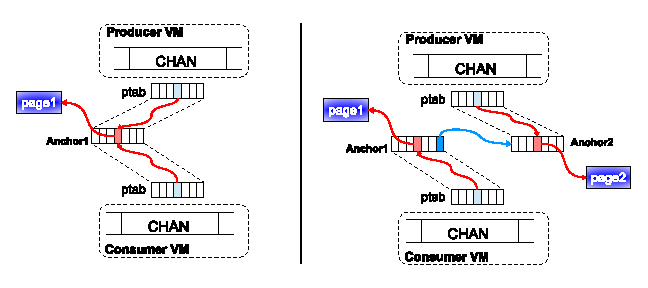
\includegraphics[width=0.45\textwidth]{eps/chan_extend.eps}
	\caption{channel extend machanism}
	\label{fig:spmckern:extend}
\end{figure}

%extension
Initially, as shown in Figure \ref{fig:spmckern:extend}(a), the runtime will not allocate the actual page frames for \code{CHAN} area but map it to a special page frame--- anchor page table (\code{Anchor1}) which is shared by the producer and consumer.
Meanwhile, each entry in the \code{ptab} of both the producer and consumer will point to the same entry in \code{Anchor1}. 

%That is each entry(pte) in \code{ptab} points to the address of Anchor1(Anchor1 in Figure\ref{fig:spmckern:extend}(a)).
When the producer sends data, the runtime attempts to write the sent data into the \code{CHAN} area, which will trigger a pagefault. 
%writing the data to CHAN, a pagefault will take place.
Then the pagefault handler will allocate a page frame (\code{page1}) for the producer, and the corresponding \code{pte} in \code{Anchor1} will be updated to point to the allocated page (\code{page1}). 
%After that, the runtime can copy the sended data to the page(\code{page1}).
%Then producer can locate the page by \code{pte} and the data need to send will copy to this \code{page1} lastly.
After that, the consumer can locate the page frame \code{page1}  and then read data from \code{page1} by by the anchor page (\code{Anchor1}).


In general producer-consumer model, if the channel buffer is full, the producer needs to wait until the consumer removes the data from it, which limits the performance and throughput of the system.
To avoid the producer waiting, we design a channel buffer with unbounded size  by exploiting an \codet{extend} mechanism\cite{zhang13lazy}.
This mechanism allows the producer uninterruptedly sending data with no need for waiting.
This \codet{extend} mechanism (Figure  \ref{fig:spmckern:extend}(b)) will remap the channel buffer (i.e., \code{CHAN} area) to another anchor and allocate some new page frames for the producer. 
At the same time, the consumer will not be disturbed and it can continuously read the data from the original page frames.
%Then the runtime will allocate the page frame(\codet{page2}) for the producer, which will be recorded in corresponding \code{Anchor2}'s PTE.
To record and trace the original  and  new page frames, an extension pte is introduced (\code{extension\_pte}).
When the consumer receives all data from the original page frames, it will locate the new page frames by the \code{extension\_pte}.
The original page frames will decrease their reference counts and are automatically freed  when the counts reach zero.



In conclusion, we design a scalable thread model (\myth) and provide an unbounded \chan for threads to communicate. This unbounded \chan is a prominent feature of \myth, which is the main difference between our \myth and the previous works. 
We will detail how to sufficiently exploit this feature to implement the scalable MapReduce (\myds)  in Section 4.
%That means a sender can send any number of messages without blocking or waiting.
%As a result, system can achieve high throughput.
%Unboundedness goal is the key to achieve high throughput.









\section{Implementation and Runtime}
In this section we discuss our extensions to 
the MapReduce programming model and shows the major changes to runtime to 
support \myds
to support pipelining between Map and Reduce (Section 3.2). 
We describe how our design supports
piplelining (Section 3.3), and discuss the buffer design (Section 3.4). 
Our focus here is on Producer-Consumer model; 
We defer performance results to Section 5.
e


\subsection{Execution flow}
\begin{figure}[!h!t]  
    \centering
    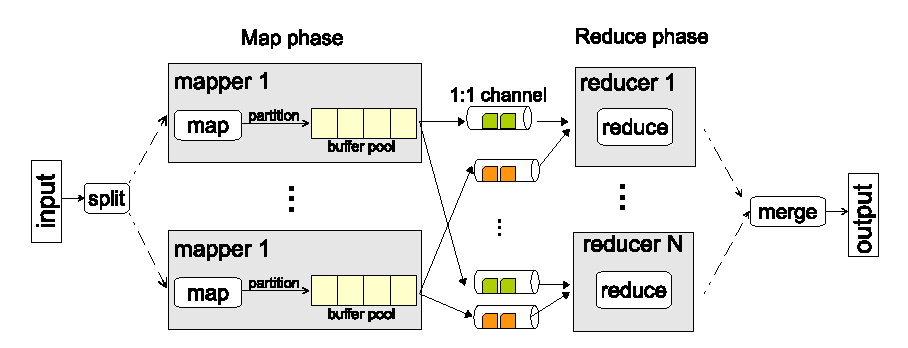
\includegraphics[width=0.5\textwidth]{eps/dmr_workflow.eps}
    \caption{The workflow of DMR}
    \label{fig:dmr:workflow}
\end{figure}

%不同与Phoenix,DMR将任务队列静态的划分给每个map worker,这样做的好处是,可以避免多个map worker对对任务队列操作从而产生锁的开销。
\myds’s implementation of MapReduce closely resembles Phoenix’s. 
There is a single master managing a number of slaves worker. 
Figure\ref{fig:dmr:workflow} illustrates the workflow of \myds,
including three main phases: map, reduce, and merge. 
At the beginning, a split function divides the input
data across workers. 
On multi-core CPUs, a worker is handled by one thread. 
A worker usually needs to process multiple input elements. 
Thus the map function is applied to the input elements one by one. 
Such an operation of applying the map function for an input element is 
called a map operation. 
Each map operation produces intermediate key-value pairs. 
Then a partition function is applied to these key-value pairs. 
Then in the reduce phase, each reduce operation
applies the reduce function to a set of intermediate pairs
with the same key. 
Finally the results from multiple reduce workers are merged and output.

Compared with existing work, 
our \myds has two main designment to improve its performance and scalability.
On the one hand, We propose produce-conumse model to 
pipeline map and reduce phase. 
ie. map worker as a producer insert key-value into local buffer,
and reduce worker as a consumer will fetch key-value from buffer
when the buffer is full. 
Reduce phase can start without waiting the Map phase finished.
On the other hand, \myds use process instead of threads, 
to avoid contention on the mm\_struct semaphores.

%The map phase reads the task’s split from task queue,
%parses it into key-value pairs, and applies
%the map function to each record.
%Intermediate keys are assigned
%to reducers by applying a partitioning function
%A spill of the in-memory buffer involves first sorting
%the records in the buffer by partition number and then by
%key.

%After receiving its partition from all map outputs, the
%reduce task enters the sort phase. The map output for
%each partition is already sorted by the reduce key. The
%reduce task merges these runs together to produce a sin-
%gle run that is sorted by key. The task then enters the
%reduce phase, in which it invokes the user-defined reduce
%function for each distinct key in sorted order, passing it
%the associated list of values.
%
%We addressed these issues by buffering the mapper output until
%it reaches a certain record threshold.
%When the record threshold isreached, 
%the mapper sends the output to a reducer. 
%Next, Reducer receives its partition from all map, 
%and enters the sort phase.
%将之前对combiner和merge阶段的特征进行简单的总结
{\bf Combiner.}
In order to maximally reduce memory pressure due to intermediate key-value
storage.%通道的数据流通量(map和reduce见传递的数据量)
%做法,开销,优势,我们的特点,可以在reduce阶段进行combiner
The imbalance of tasks can be solved by dynamic scheduling in the Map phase. 
%%事实上,为了防止出现数据倾斜的问题,即map阶段的很多key都发送到一个reduce,导致某个reduce有过多的动态内存分配,甚至可能出现内存不够的情况,我们可以对reduce的数据做局部的combiner
%However, in the Reduce phase, 
%as all values for the same key must be in one reduce task, 
%it is not always feasible to generate a large number reduce tasks for
%%dynamic scheduling.

{\bf merge.}
Each Reduce generates a set of output key/value
pairs, and the library’s Merge phase sorts them by key to
produce the final output. 
%做法,作用,我们的优化,不需要进行reduce和merge的阶段,应当尽量避免,以降低时间的开销

\subsection{Pipelined execution}
Pipelined map and reduce has been adopted 
in the MapReduce framework for distributed computing\cite{Condie2010MapReduce,}. 
Condie et al. show that since the intermediate data is delivered to
downstream operators more promptly, 
it is able to improve resource utilization.

%In general MapReduce programming model, 
While in Phoenix, (To avoid mulit map and reduce contention the same area, )
there is a strict barrier between the Map and Reduce phases: 
the workers in one phase can only be started 
until all workers in the previous phase has been finished. 
Hence, the execution time of a job is determined by the
slowest worker in each phase. 
A downstream dataflow element can begin consuming data
before a producer element has finished execution, which can
increase opportunities for parallelism, improve utilization,
and reduce response time.
On the other hand, MapReduce workloads
are an ideal candidate for pipelining as the user-defined
map functions are usually computation-intensive, while the
reduce phase to construct the global container is memory
intensive\cite{talbot2011phoenix++}.
Overlapping the
computation-intensive and memory-intensive workloads 
can effective improve the overall hardware resource utilization.

%我们设计了一个生产者和消费者模型,用于map和reduc阶段的流水并行,有两个重要的数据结构:map worker的buffer池,reducer worker的全局buffer。每个map worker拥有一个私有的buffer池,当key-value产生后,通过partition函数插入到对应的buffer中。其中每个buffer对应一个reduce worker,reduce worker轮循的从各个map的buffer池中取key-value,并调用reduce函数进行计算;每个reduce拥有一个私有的全局buffer,用于存放reduce处理后得到的全局结果。
We design a producer-consumer model to pipeline the
map and reduce phases.
There are two major data structures,
which are local buffers pool for each map worker and 
a global buffer for reduce worker.
Specifically, 
each map worker has a local buffers pool and 
each buffer for a corresponding reduce worker.
Partition function will be used to push key-value into a corresponding
buffer.
When the buffer threshold is reached,
the corresponding reduce worker can read record in the buffer.
One reduce worker will get key-value from each map by Round-Robin and 
merge the key-value pairs to the global buffer.


%如同Phoenix, 默认情况下,buffer使用hash table来实现,事实上,在我们的模型中,使用array来实现具有更好的性能。下面的章节会详细解释原因。
Defaultly, the buffer is a hash table as Phoenix.
While this technique is more effective for the array buffer
container than the hash buffer. 
We will explain the advantage of array buffer in section 3.2.1.
MRPhi\cite{lu2013mrphi} is also use producer-consumer model to 
pipeline the map and reduce phases. 
There are partitions queues for each reduce worker.
While we don't use queues, mapping will be used in DMR(section 3.2.2).

%(The motivation is that the map function defined by users
%usually performs heavy computation. But the reduce phase
%contains many memory accesses in which the major work is to
%construct the global container. 
% )


\subsubsection{Producer-Consumer model}
The pipelined map and reduce are implemented using a
producer-consumer model. 
The map and reduce workers are the producers and consumers, respectively.
Specially, the map worker generate key-value and 
put it into the buffer.
At the same time, 
the reduce worker is consuming the key-value.
%由于map和reduce worker共享这个buffer,因此最关键的问题是如何同步
As the buffer is a shared region of memory in tradition,
either a map worker or a single reduce worker,
can access the structure at any given time.
%使用queue
In fact, producer-consumer model implementations
often use a shared queue.

MRphi\cite{lu2013mrphi}design a producer-consumer model 
to pipeline the map and reduce phases. 
There are three major data structures, 
which are local hash tables, a global hash table, 
and partition queues. 
Specifically, each map worker has a local hash table. 
When a local hash table is full,
key-value pairs stored in this table are partitioned and
pushed into corresponding queues. 
Meanwhile, one reduce
worker works on one queue to merge the key-value pairs to
the final global hash table.
% MRPhi的缺点,(1)多对一的竞争问题,(2)队列的管理问题
{\color{red}They don’t describe, however, how to manage the queue,
which allocted a space or use malloc}


There three differences DMR and MRphi:
(1) when the map local hash table is full,
key-value pairs stored in this table are partitioned and
pushed into corresponding queues.
%hash table 数据分布不均匀,如果只是简单的做一个 partition,可能导致有些 reduce task很小,甚至为空。而每次的将 reduce task 加入到 queue 都需要同步的开销
(2) when map worker insert reduce taskes to the queue of reduce,
the map worker is stoped to wait.
%map worker 将 reduce task 插入到 queue 这个过程,需要停下来等待,无形中延迟了 map 的执行时间
(3)%多个 map worker 会同时对 reduce worker 的 queue 进行操作,需要相应的同步手段,由此会产生等待开销。核数越多,开销会越明显。
As the queue of reduce worker will be operation by multi map worker,

t is important for databases and large web and proxy servers to map files into memory instead of having a buffer and reading the file contents into the buffer. If you map the file into memory directly, the operating system has more memory left for I/O buffering.


Figure\ref{fig:dmr:spmc}
\begin{figure}[!h!t]
    \centering
    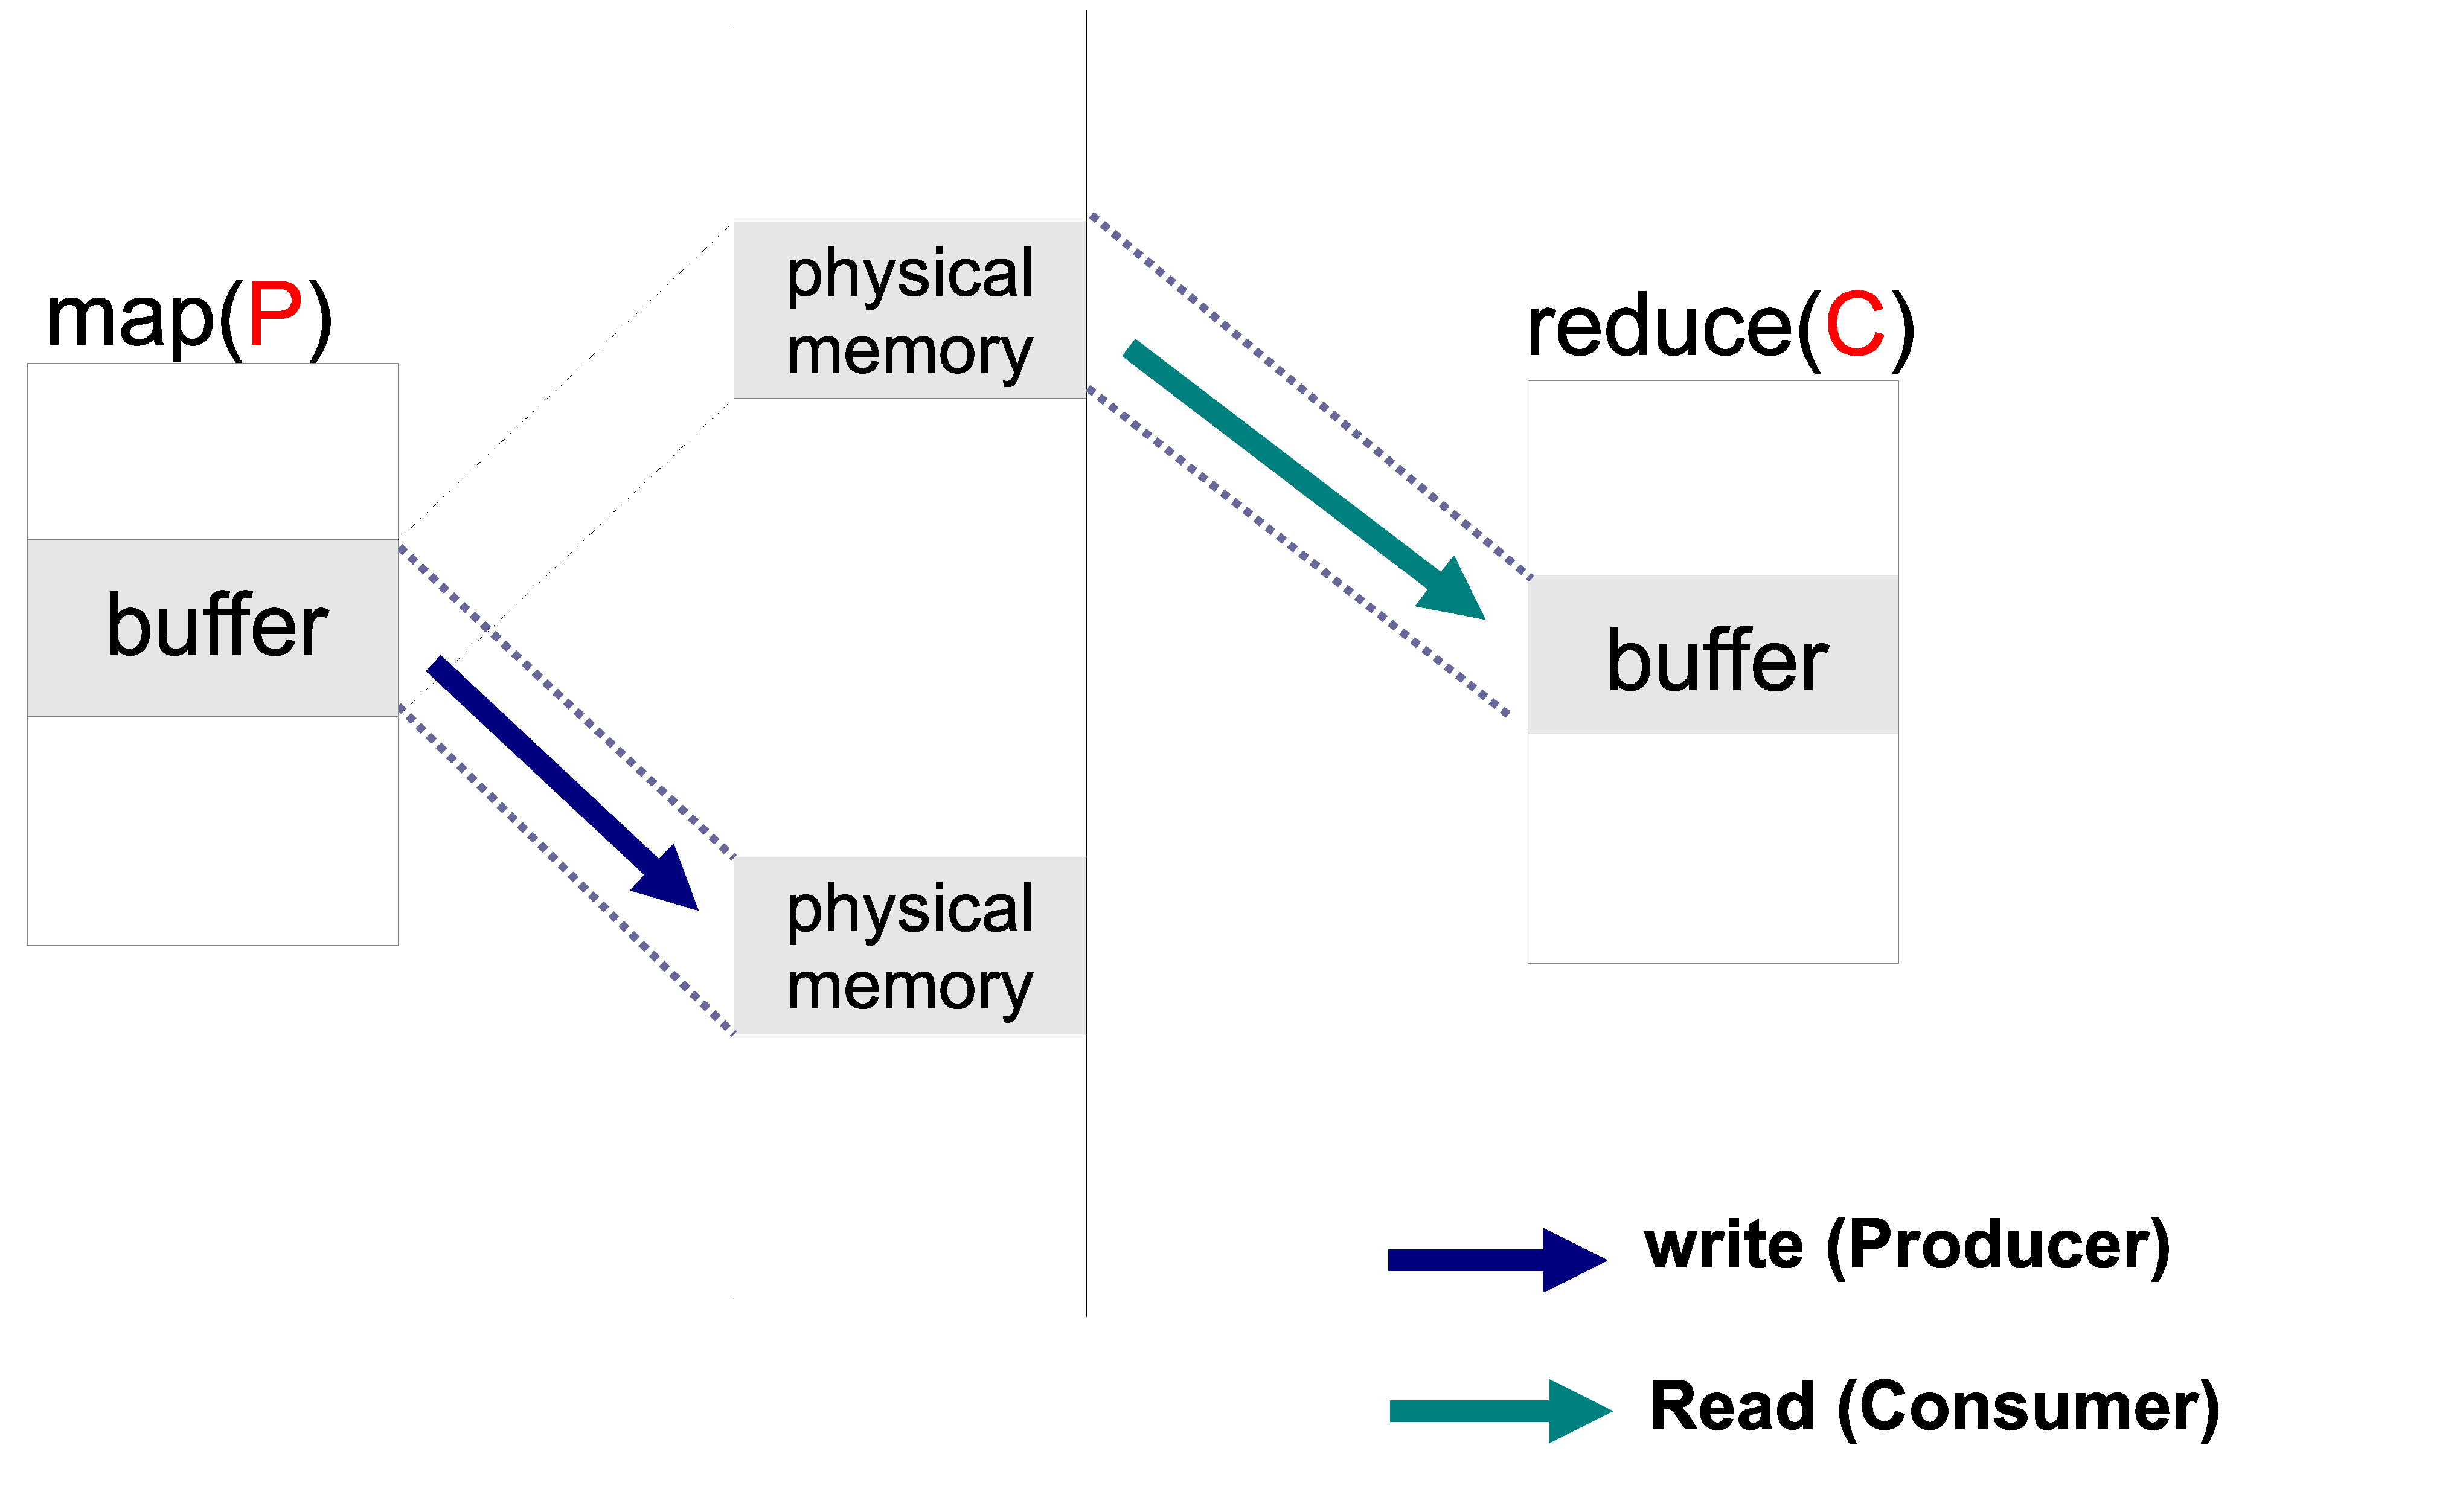
\includegraphics[width=0.45\textwidth]{eps/dmr_pc_model.eps}
    \caption{producer-consumer model}
    \label{fig:dmr:spmc}
\end{figure}
%SPMC的快速
{\color{gray}
In the shared-memory model, a region of memory that is shared
by cooperating processes is established. 
Processes can then exchange information 
by reading and writing data to the shared region.
Shared memory can be faster.
since in shared-memory systems, system calls are required only to establish shared-memory regions. 
Once shared memory is established, all accesses are treated
as routine memory accesses, and no assistance from the kernel is required.
}
%SPMC区域的建立
Interprocess communication using shared memory requires communicating
processes to establish a region of shared memory. Typically, a shared-memory
region resides in the address space of the process creating the shared-memory
segment. Other processes that wish to communicate using this shared-memory
segment must attach it to their address space. 

%SPMC区域的使用,对应buffer
To allow producer and consumer processes to run concurrently, we must have
available a buffer of items that can be filled by the producer and emptied by
the consumer. This buffer will reside in a region of memory that is shared by
the producer and consumer processes.(http://bulk.fefe.de/scalability/)

\subsubsection{Extention of SPMC}


\input buffer


\subsection{Separate Address Space}

One reason that widely used operating systems use a lock on the address space is that 
they use complex index data structures to guarantee O(log n)
lookup time when a process has many mapped memory
regions. Linux uses a red-black tree for the regions [27],
FreeBSD uses a splay tree [1], and Solaris and Windows use
AVL trees [24, 29]. 
Because these data structures require re-
balancing when a memory region is inserted, they protect the
entire data structure with a single lock.


%先详细分析Phoenix使用线程存在的问题,然后我们采用进程地址空间隔离会有哪些好处
%虽然MRPhi中也是使用producer-consumer model,DMR不同之处在于,(1)它不需要显示的管理map和reduce间的队列,简单;(2)
In addition to global locks like the ones discussed earlier, 
data structure private locks can also be a problem 
if the data structure is shared by multiple threads. 
A standard example here are the mm\_sem read-write semaphore 
that protects the list of mappings in a process and 
the pagetable\_lock that protects the pagetable state of a process. 
These locks are local to a process’ address space. 
However when the process is using multiple threads 
then these threads will be able to access the address space in parallel,
which can cause contention on these locks. 
A classical example here is 
the initialization of a large multi-threaded computing job 
that causes a lot of parallel page-faults. 
These page-faults will all run into contention on the mm\_sem semaphores. Semaphores are sleeping locks 
and may run into convoying problems 
where waiting threads may 
get stuck at the end of the wait queue for a long time.\cite{Andi2009lmulticore}

Unfortunately these programs are often written to start as many threads as the system has CPUs, 
but when the system is larger than their scalability limit adding more threads might actually scale negatively.
The first measure is to limit them to the maximum number of threads that they can successfully scale to.
This of course leaves some of the CPUs idle. 




There is a sense in the community that traditional kernel
designs won’t scale well on multicore processors: that
applications will spend an increasing fraction of their time
in the kernel as the number of cores increases.

To understand the Linux scalability
behavior, we analyze the related implementation of Linux
kernel and exploit performance tools to identify scalability
bottlenecks.


As indicated by this figure, the time of completing
a workload for one core increases when there are more
cores in the system. The trend of this curve suggests that
the parallel scalability of forkbench is poor.

In order to understand the scalability behavior, 
Perf\cite{} is exploited to collect execution time information
on the function basis. 
Experimental results on 32 cores
show that \_\_ticket\_spin\_lock and 
default\_send\_IPI\_mask\_sequence\_phys are two functions 
which have largest execution time with 71.25\% and 10.20\% respectively. 

Performance data reveal that two functions vma link() and
unlink file vma() have the largest execution time (46.02%
and 49.97\%) and lock contention. Call-graph information
and source code analysis show that the two functions are
called when adding a virtual memory address range into the
process address space or deleting a virtual memory address range. 
When multiple slave processes call mmap() or unmap() concurrently, the 
memory mapped file address range should be added into or 
deleted from each slave process address space. However, 
the same spin lock protecting the memory mapped file 
address range should be held or released. Thus, spin lock 
contention degrades the parallel scalability performance of 
the benchmark. 



The difference between processes and threads under Linux 2.4 is that threads share more parts of their state (address space, file handles etc) than processes, 

\section{Evaluation}
We evaluate \myds and Phoenix on 
a 32-core Intel 4× Xeon E7-4820 system equipped with 128GB of RAM. 
The operating system is Ubuntu 12.04 with kernel 3.2.0 and glibc-2.15.
Benchmarks were built as 64-bit executables with gcc -O3.
We logically disable CPU cores using Linux’s CPU hotplug mechanism, 
which allows to disable or enable individual CPU cores 
by writing “0” (or “1”) to 
a special pseudo file (/sys/devices/system/cpu/cpuN/online), 
and the total number of threads was matched to the number of CPU cores enabled.
Each workload is executed 10 times. 
To reduce the effect of outliers, 
the lowest and the highest runtimes for each workload are discarded, 
and thus each result is the average of the remaining 8 runs.

%\subsection{ Performance Improvements Summary}
\subsection{Performance of benchmarks}
%描述benchmarks的特点,benchmarks的数据集等

\begin{figure*}[htpb]
\centering
  \subfigure[SMR versus Phoenix with ptmalloc]{
   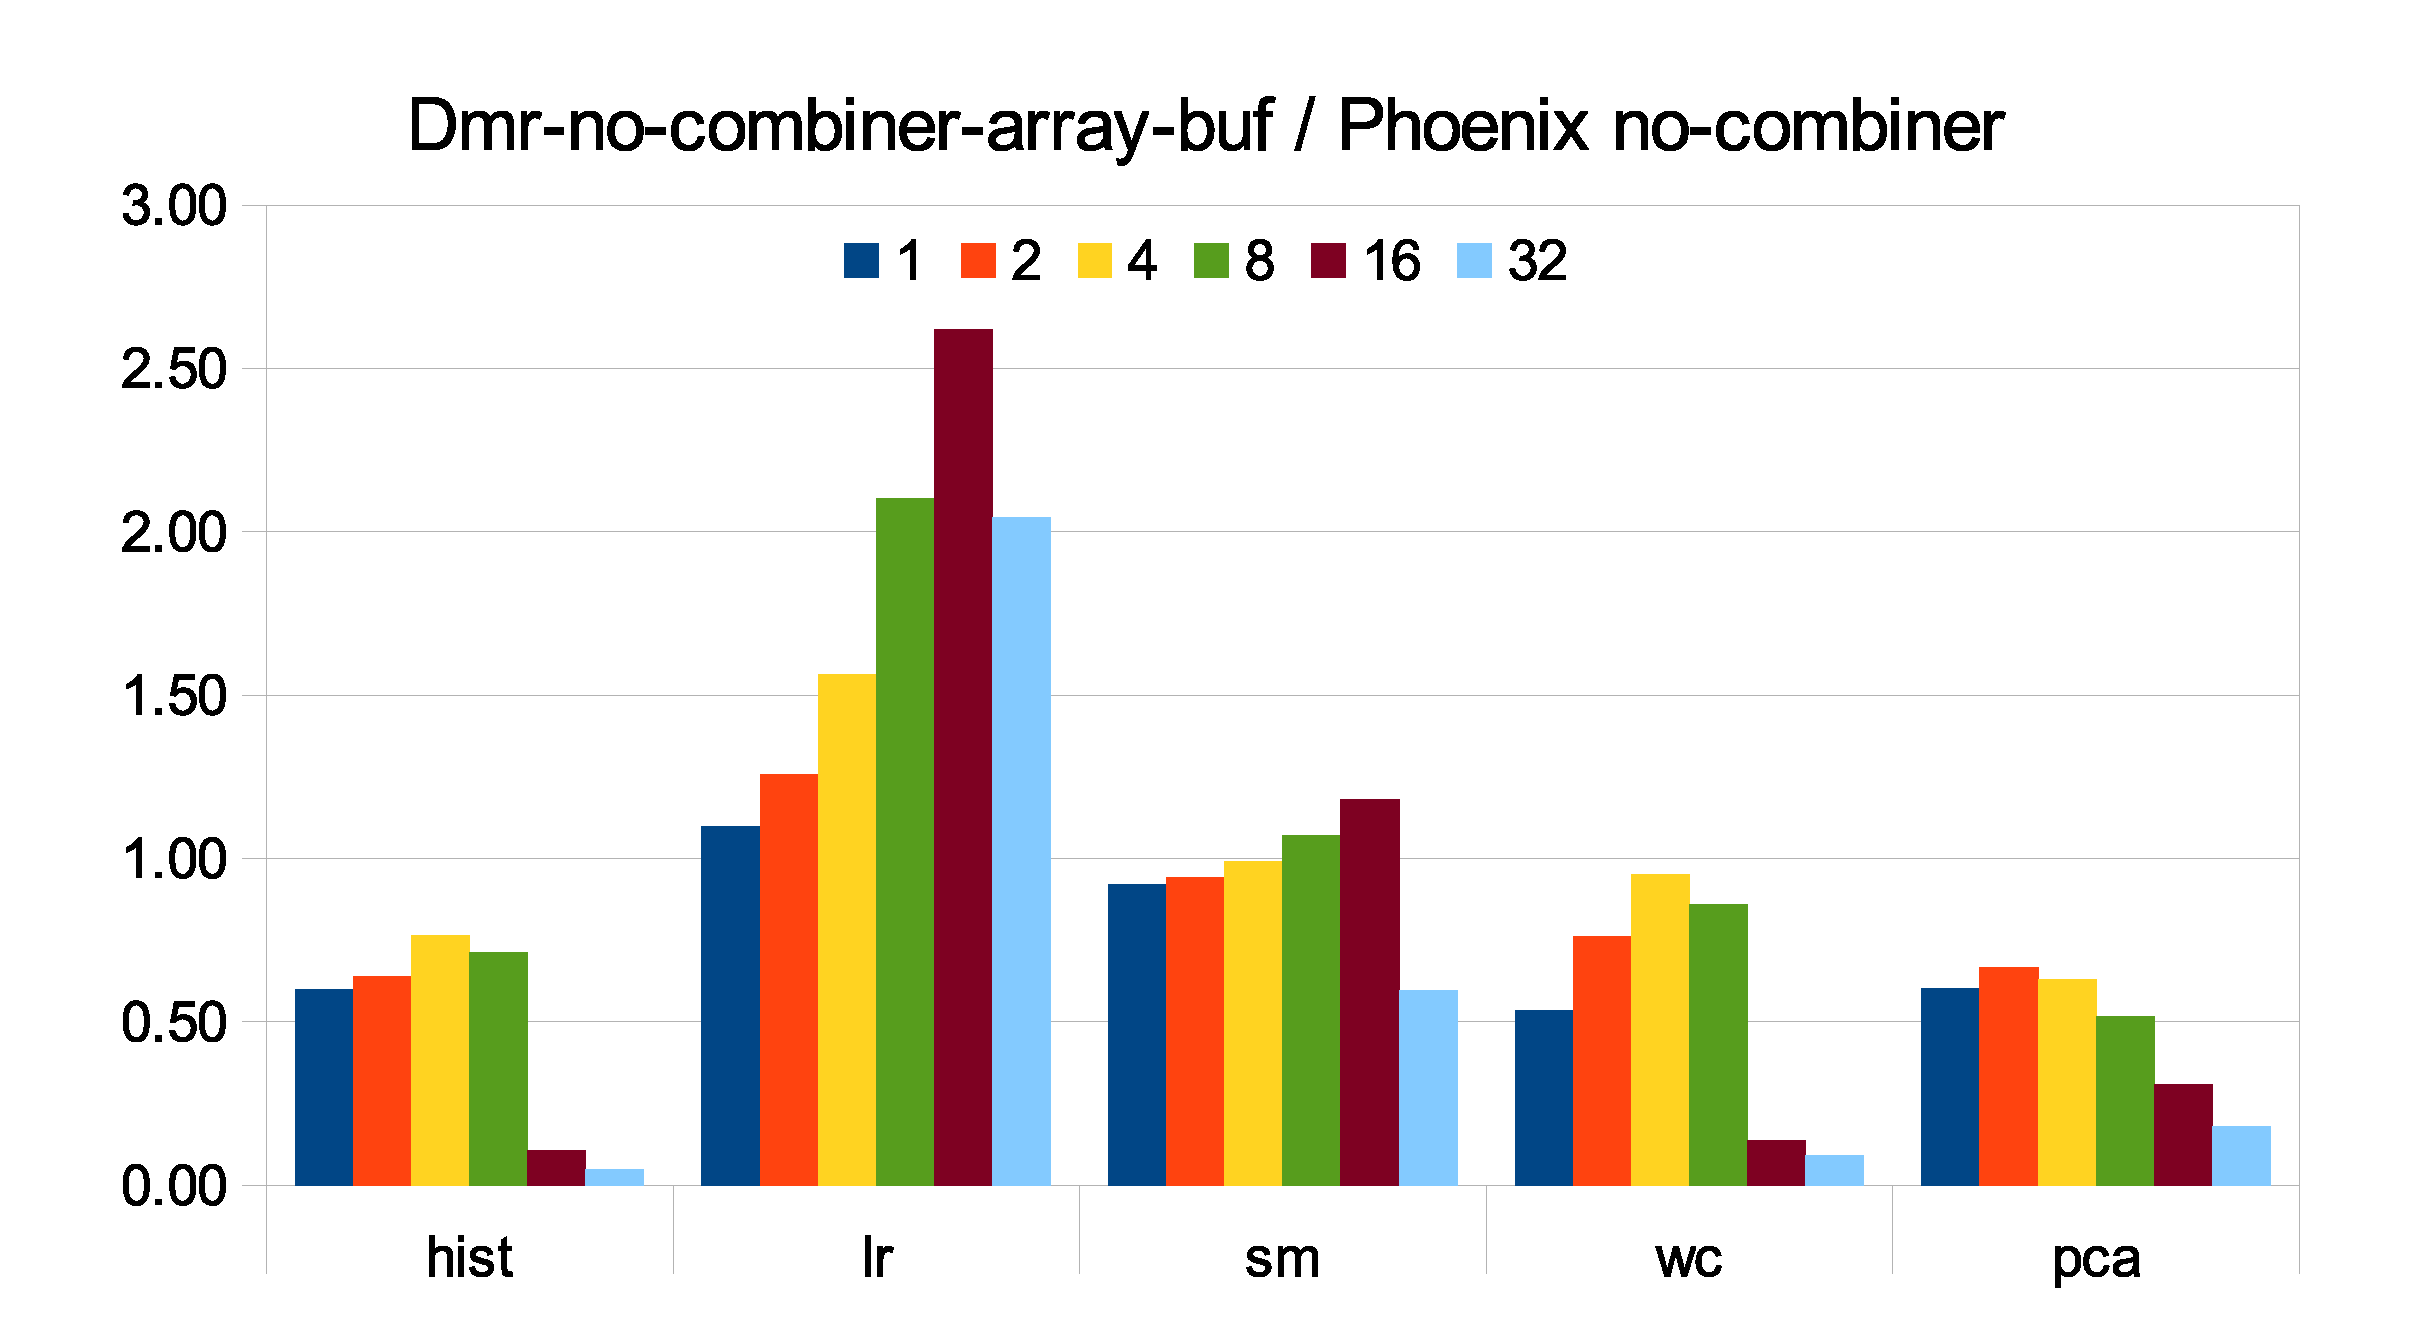
\includegraphics[width=0.45\textwidth]{eps/dmr_time_array.eps}
   \label{fig:dmr:time:ptmalloc}
  }
  \subfigure[SMR versus Phoenix with jemalloc]{
   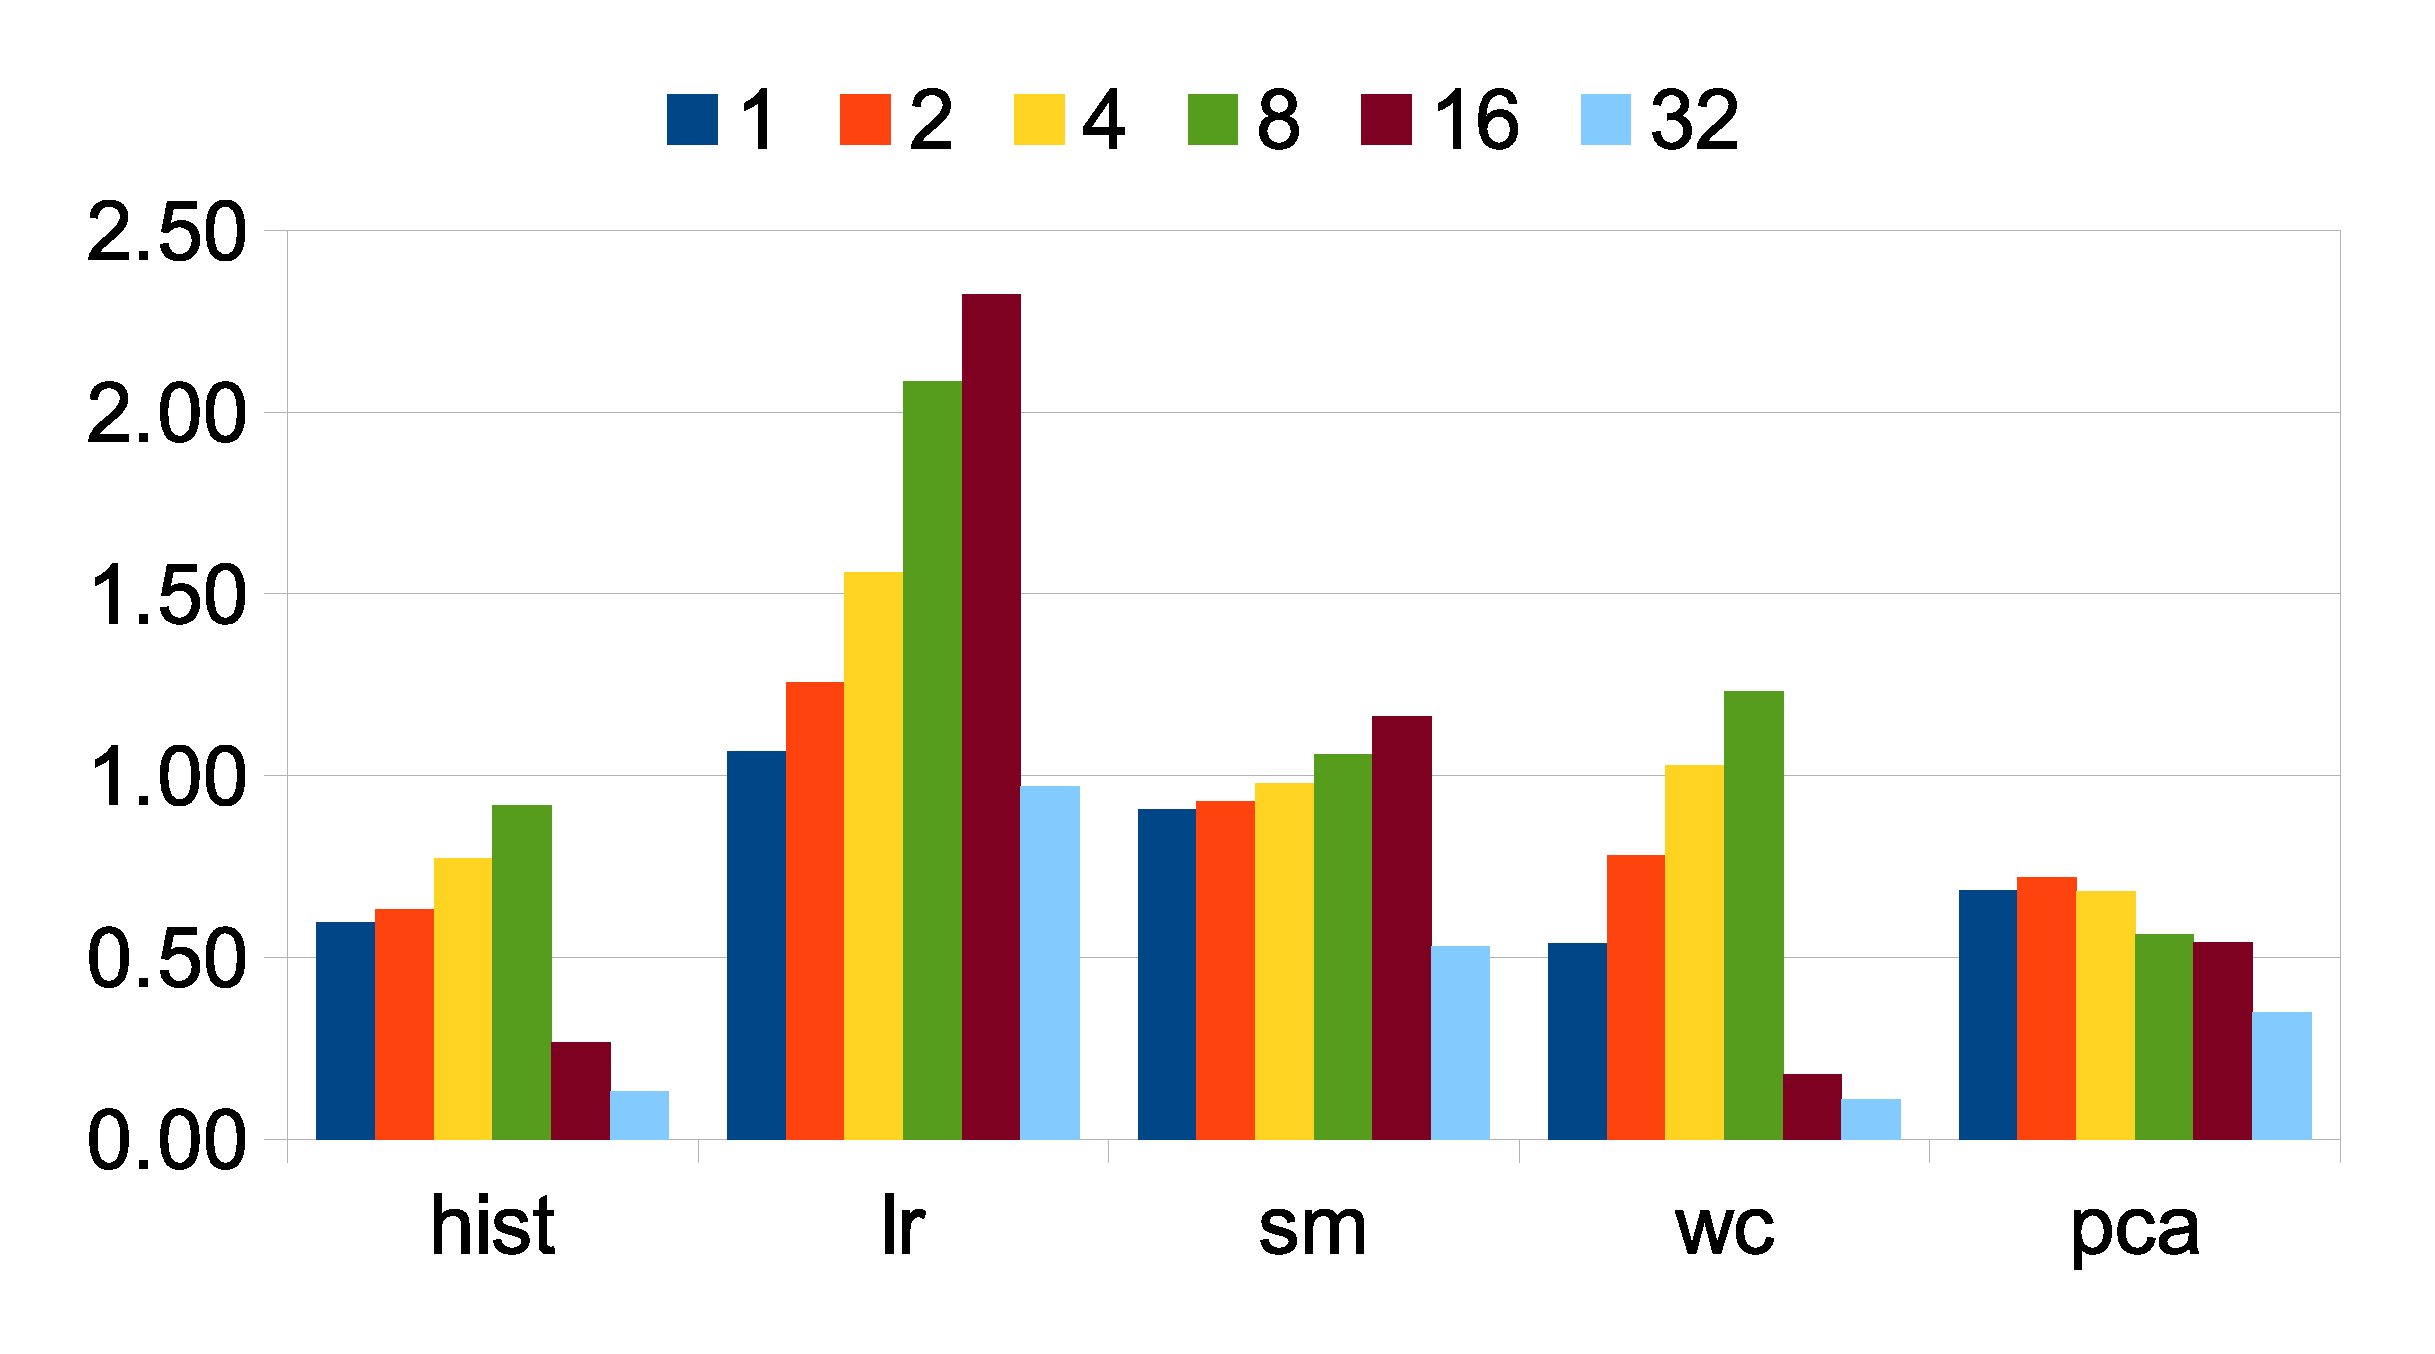
\includegraphics[width=0.45\textwidth]{eps/dmr_time_jemalloc.eps}
   \label{fig:dmr:time:jemalloc}
  }
  \caption{Execution time of SMR versus Phoenix}
   \label{fig:time}
\end{figure*}

{\bf Performance}
We measured \myds performance by executing the applications
included in the original release. 
\grayt{Table II describes the workloads and their input datasets. 
Compared to Phoenix, we significantly increased the performance.
However, some of the workloads still did not scale particularly well. 
We discuss their bottlenecks in detail in Section 5, 
but in the remainder of this section 
we first focus on the optimizations that turned out to be successful.
}
We experimented with various allocators.
Since there are many heap objects shared among threads
in Phoenix, and it is sensitive to memory allocator.
Compared to the libc sequential allocator ,  
ptmalloc\cite{gloger1997ptmalloc},
jemalloc{evans2006jemalloc} provided improved performance. 
the memory allocator in glibc, does not scale on multicore system. 
Therefore we evaluate the Phoenix with jemalloc and
compare it  with \myds(Figure \label{fig:dmr:time:jemalloc}).
Phoenix-jemalloc speedup Firgure \ref{fig:phoenix:speedup:jemalloc}

However, nether allocator could successfully scaled up to 32cores.

Figure\ref{fig:dmr:time:ptmalloc} and \ref{fig:dmr:time:jemalloc}
present the Execution time of \myds versus Phoenix.
%虽然jemalloc的性能表现要比ptmalloc好,但实验结果都显示
\myds matches or outperforms Phoenix on 4 out of 5 workloads,
but runs worse than Phoenix only on linear\_regression.
For hist, pca and word\_count, 
\myds outperforms Phoenix betwen xxx and xxx faster.
The reason of worse performance on linear\_regression 
is that most of time is waste in \myds's initailization.
We will evaluation overhead of initialization time in section\ref{}.
%从实验的结果可以看出,hist, wc, pca,SMR的性能较好,sm相当,lr中SMR的性能表现较差



\begin{figure*}[htpb]
\centering
  \subfigure[]{
   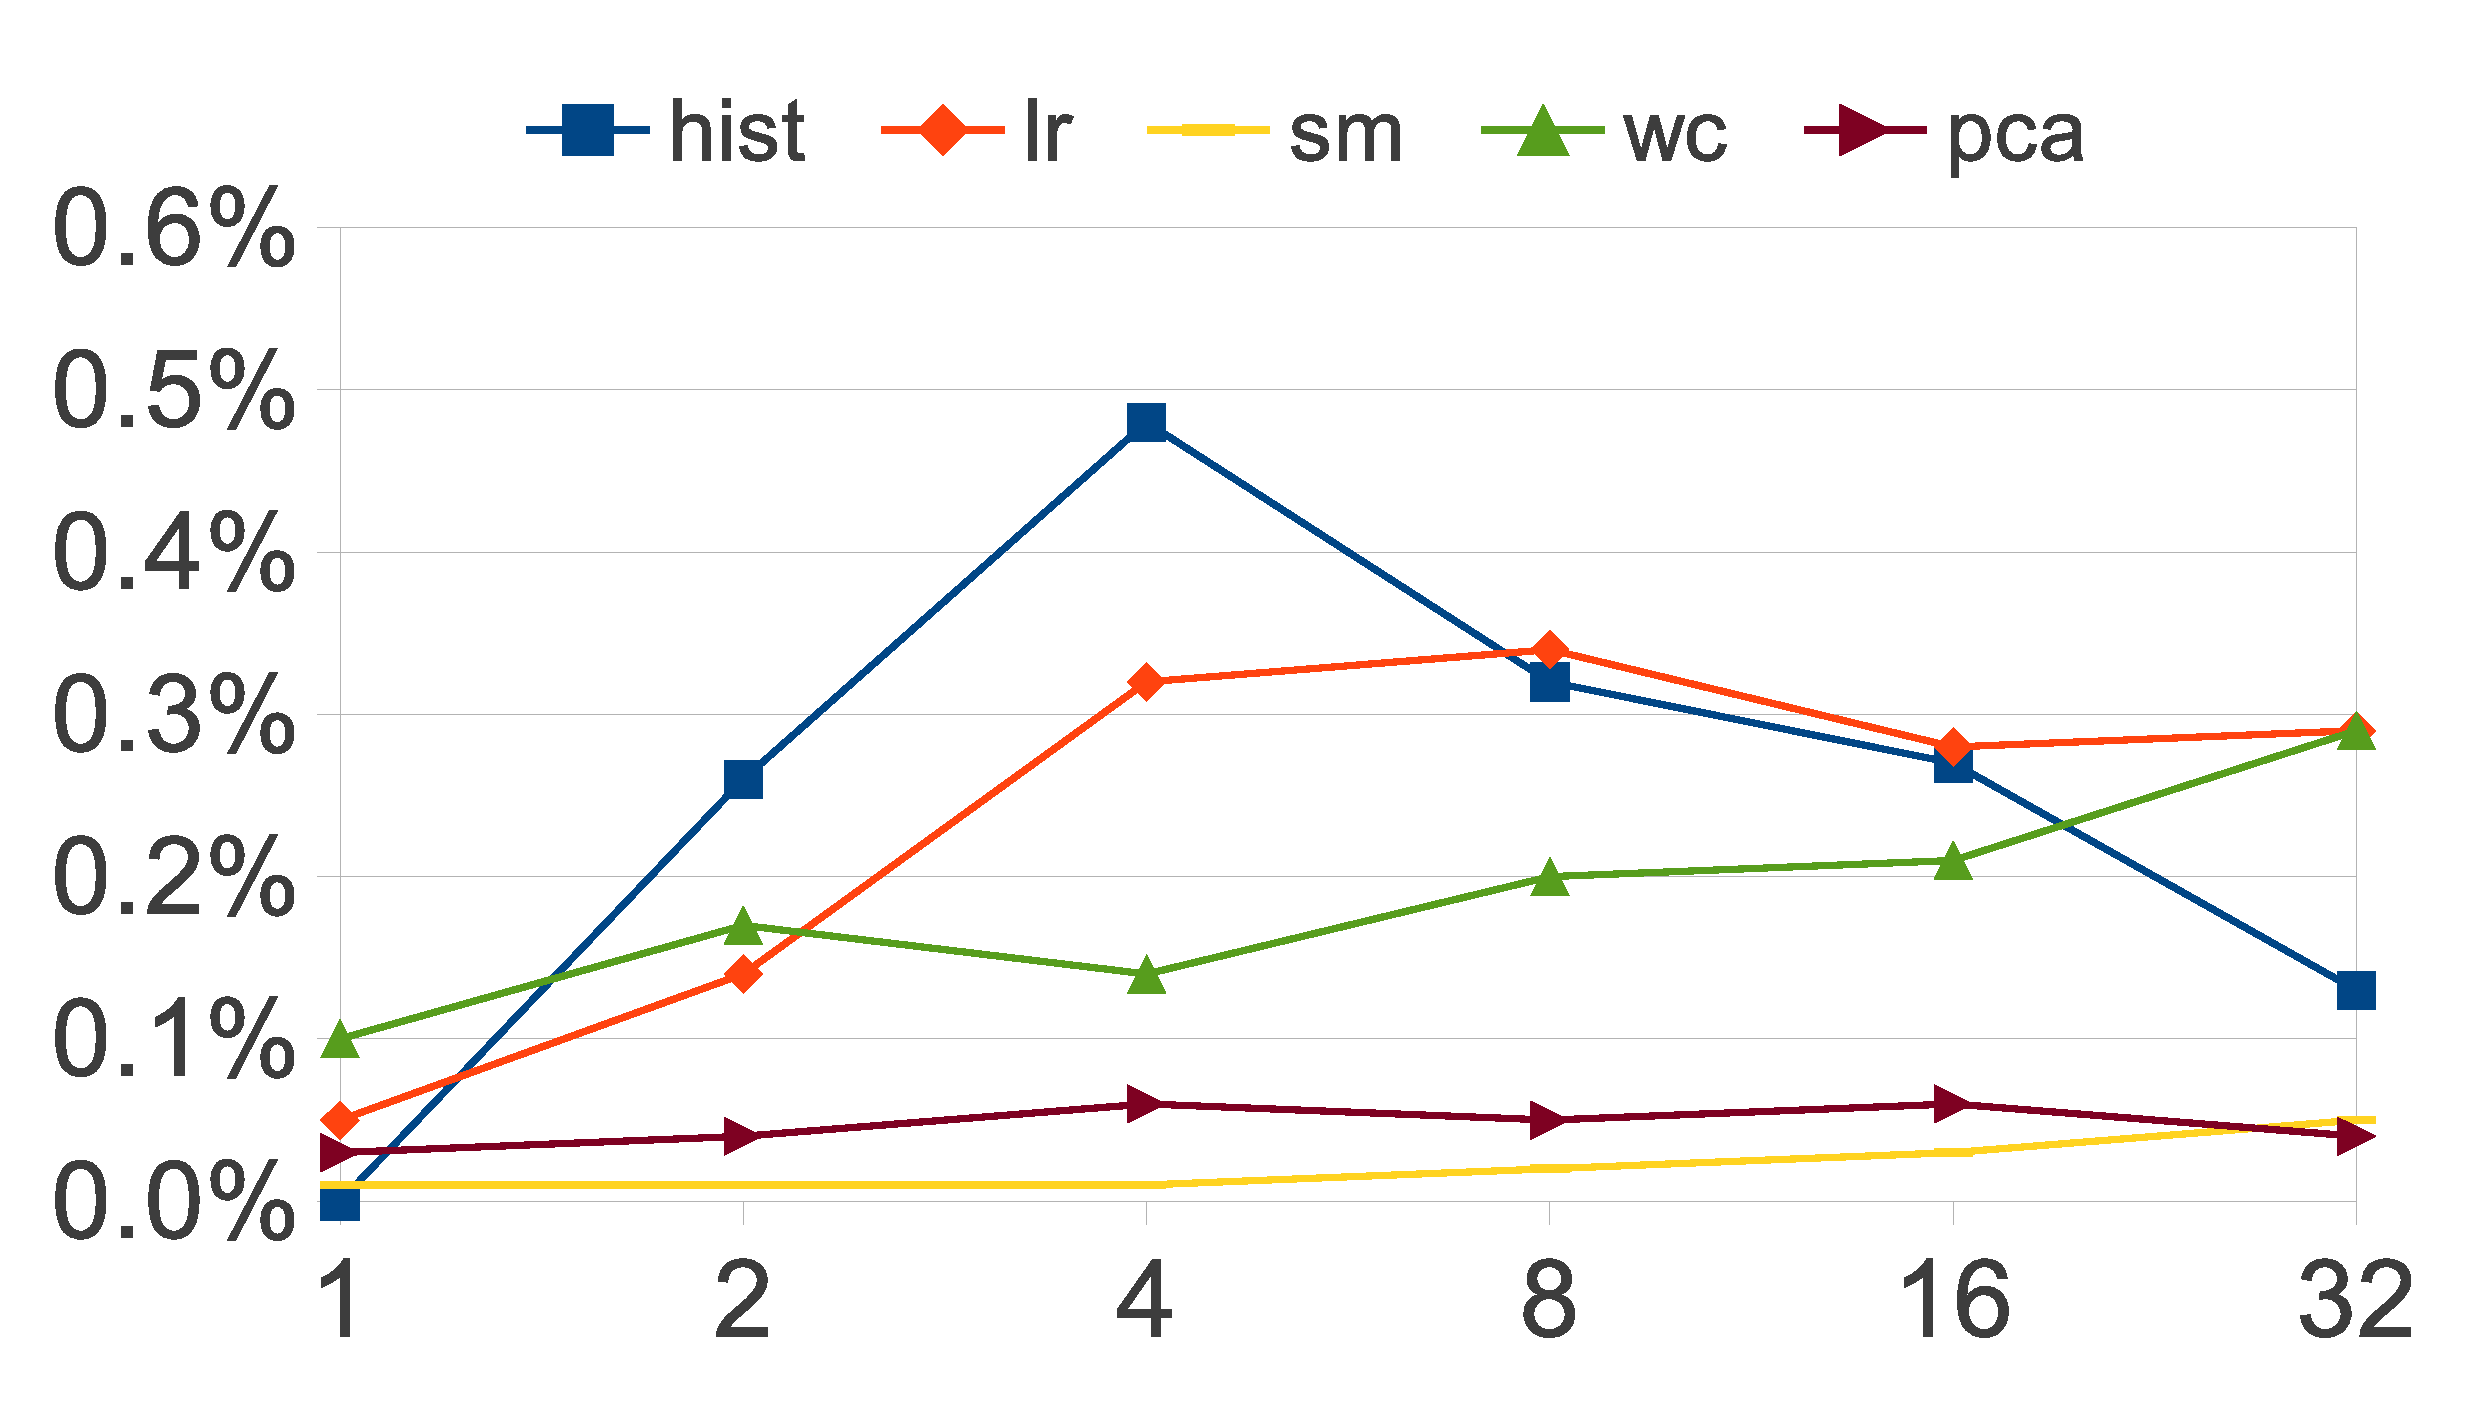
\includegraphics[width=0.45\textwidth]{eps/dmr_spinlock.eps}
   \label{fig:dmr:time:ptmalloc}
   }
  \subfigure[]{
   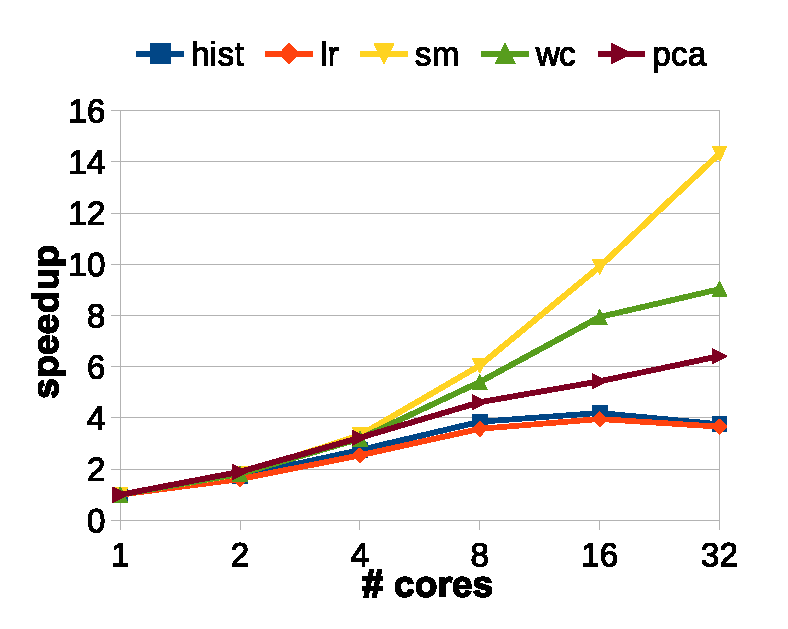
\includegraphics[width=0.45\textwidth]{eps/dmr_speedup.eps}
   \label{fig:dmr:time:jemalloc}
  }
  \caption{ Application speedup with the \myds}
   \label{fig:scalability}
\end{figure*}
{\bf Scalability}


We say a waiting thread is the thread which is waiting for shared
data that produced by another thread. If using semaphore for
synchronization, a waiting thread will be blocked and enlisted
on the waiting queue by the OS scheduler. If using spinlock
for synchronization, a waiting thread will do busy wait, i.e.
spinning in a while loop. Embedded software applications
that using semaphore to handle the synchronization could
result in performa+nce overkill, since it involves system calls
translated into thousands of CPU instructions [1]; while using
spinlock have problem of long busy-waiting time.

When a running thread tries to read shared data,
it must do busy wait until it has exhausted its time-slice
or until another thread has withdrawn the occupation on the
shared data. 




System performance is evaluated using
instructions per cycle (IPC). Higher IPC means
better performance.
Figure \ref{fig:perf:ipc} shows the IPC of Phoenix first increases 
and then decreases as more threads are run on multi-core system.


{\color{red}\myds }
Evaluation indicates that
the locking overhead can be significantly reduced to less
than 1% of total runtime on 32 cores




%分析lr性能差的原因

The performance of hist, wc, sm are scale linearly with the number of cores.


\subsection{ Impact of buffer Optimizations}
As the number of threads increases (from 1 to 8), the
execution time decreases for all cases. For 9 to 32 threads,
both Phoenix and \myds execution times keep decreasing with
the increase of the number of threads
When the number of dependent processes increases above the
number of cores, 
%context switching takes place, 
serious contending lock takes place,
and as a resultexecution time will be drastically increased. 
As the number of threads increases from 32 to 33, 
there is a significant increase
in execution time owing to Opteron’s NUMA architecture with
point-to-point communication links.

On the workstation, the \myds implementation is 13\%-
95\% better than Phoenix implementation (peaking at 8
threads).

As the number of threads increases (from 1 to 8), the
execution times for both Pthread/C and MPI programs decrease
for both workstation and supercomputer. For 9 threads to 32
threads, Pthread/C and MPI execution times changes slightly
on workstation. However for 9 threads to 32 threads, both
Pthread/C and MPI execution times keep decreasing (in most
cases) with the increase in number of threads on the
supercomputer node. This is because we use 8 cores in the
workstation while we use 32 cores in the supercomputer node.
Execution time for large number of threads (9 to 33 and
beyond) remains almost the same for the workstation because
of no communication overhead. Results (see Figure 4) also
show that MPI execution time on supercomputer increases
significantly when the number of threads is increased from 32
to 33 and beyond; but Pthread/C execution time on
supercomputer remains almost unchanged. This is due to the
communication overhead among the cores (32 cores in a
supercomputer node) when using MPI message passing.

From the
experimental results, it is observed that both computer systems
yield better performance using Pthread than MPI (in most
cases). Pthread has the advantage over MPI for sharing
memory and distributing tasks among lightweight threads
instead of processes. The performance of the Pthread
implementation on the supercomputer is the best, 30%-6.7x
better than the Open MPI implementation on the
supercomputer node.

\subsection{ Challenges and Limitations}
\begin{figure}[htpb]
\centering
  \subfigure[Execution time and initialization time on histgram]{
   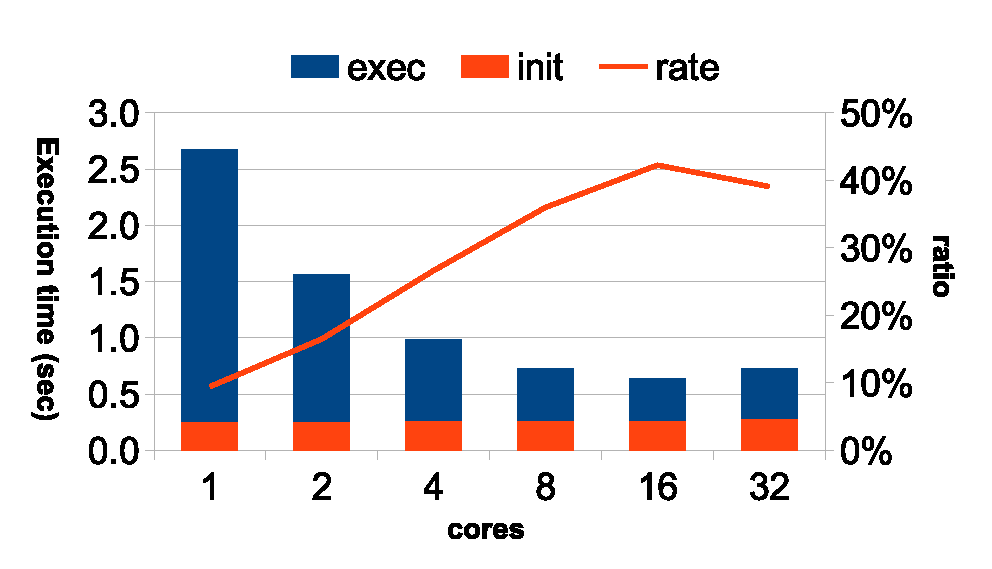
\includegraphics[width=0.45\textwidth]{eps/dmr_hist_init.eps}
   \label{fig:dmr:hist:init}
   }
  \subfigure[Execution time and initialization time on linear\_regression]{
   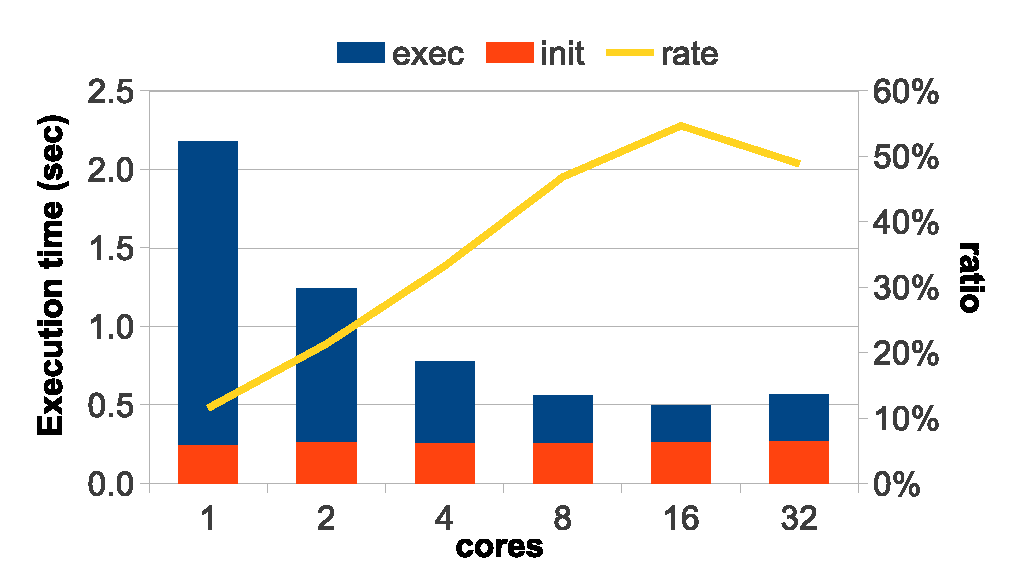
\includegraphics[width=0.45\textwidth]{eps/dmr_lr_init.eps}
   \label{fig:dmr:lr:init}
  }
  \caption{Initialize time with \myds}
   \label{fig:init}
\end{figure}
Figure\ref{fig:init} shows the initialization time of \myds and Phoenix.
The time of \myds used is range 0.25s to  0.35s, 
while it is just about 0.001s in Phoenix.
{\color{red} why the initialization time is so large in \myds}

Although we were able to significantly improve the scalability of \myds, 
workloads histogram, linear regression still did not scale up to 32cores. 
%We used /usr/bin/time to assess where the execution time was
We used stub to assess where the execution time was
being spent. 
Figure \ref{fig:dmr:hist:init} shows the result with exec time
defined as mapreduce actual execution time and init time as the initialization time before workers starting work. 
It was clear that the 2 non-scaling workloads shared two common trends. 
First, the init time ratio increased with increasing number of threads, 
dominating the total execution time at high thread count. 
%Second, the portion of actual computation time assumed by kernel code (sys /
%effective) significantly increased as we went beyond the single
%chip boundary.
%Second, both total execution time are short, While the portion of init time is 

\begin{figure}[htpb]
\centering
  \subfigure[]{
   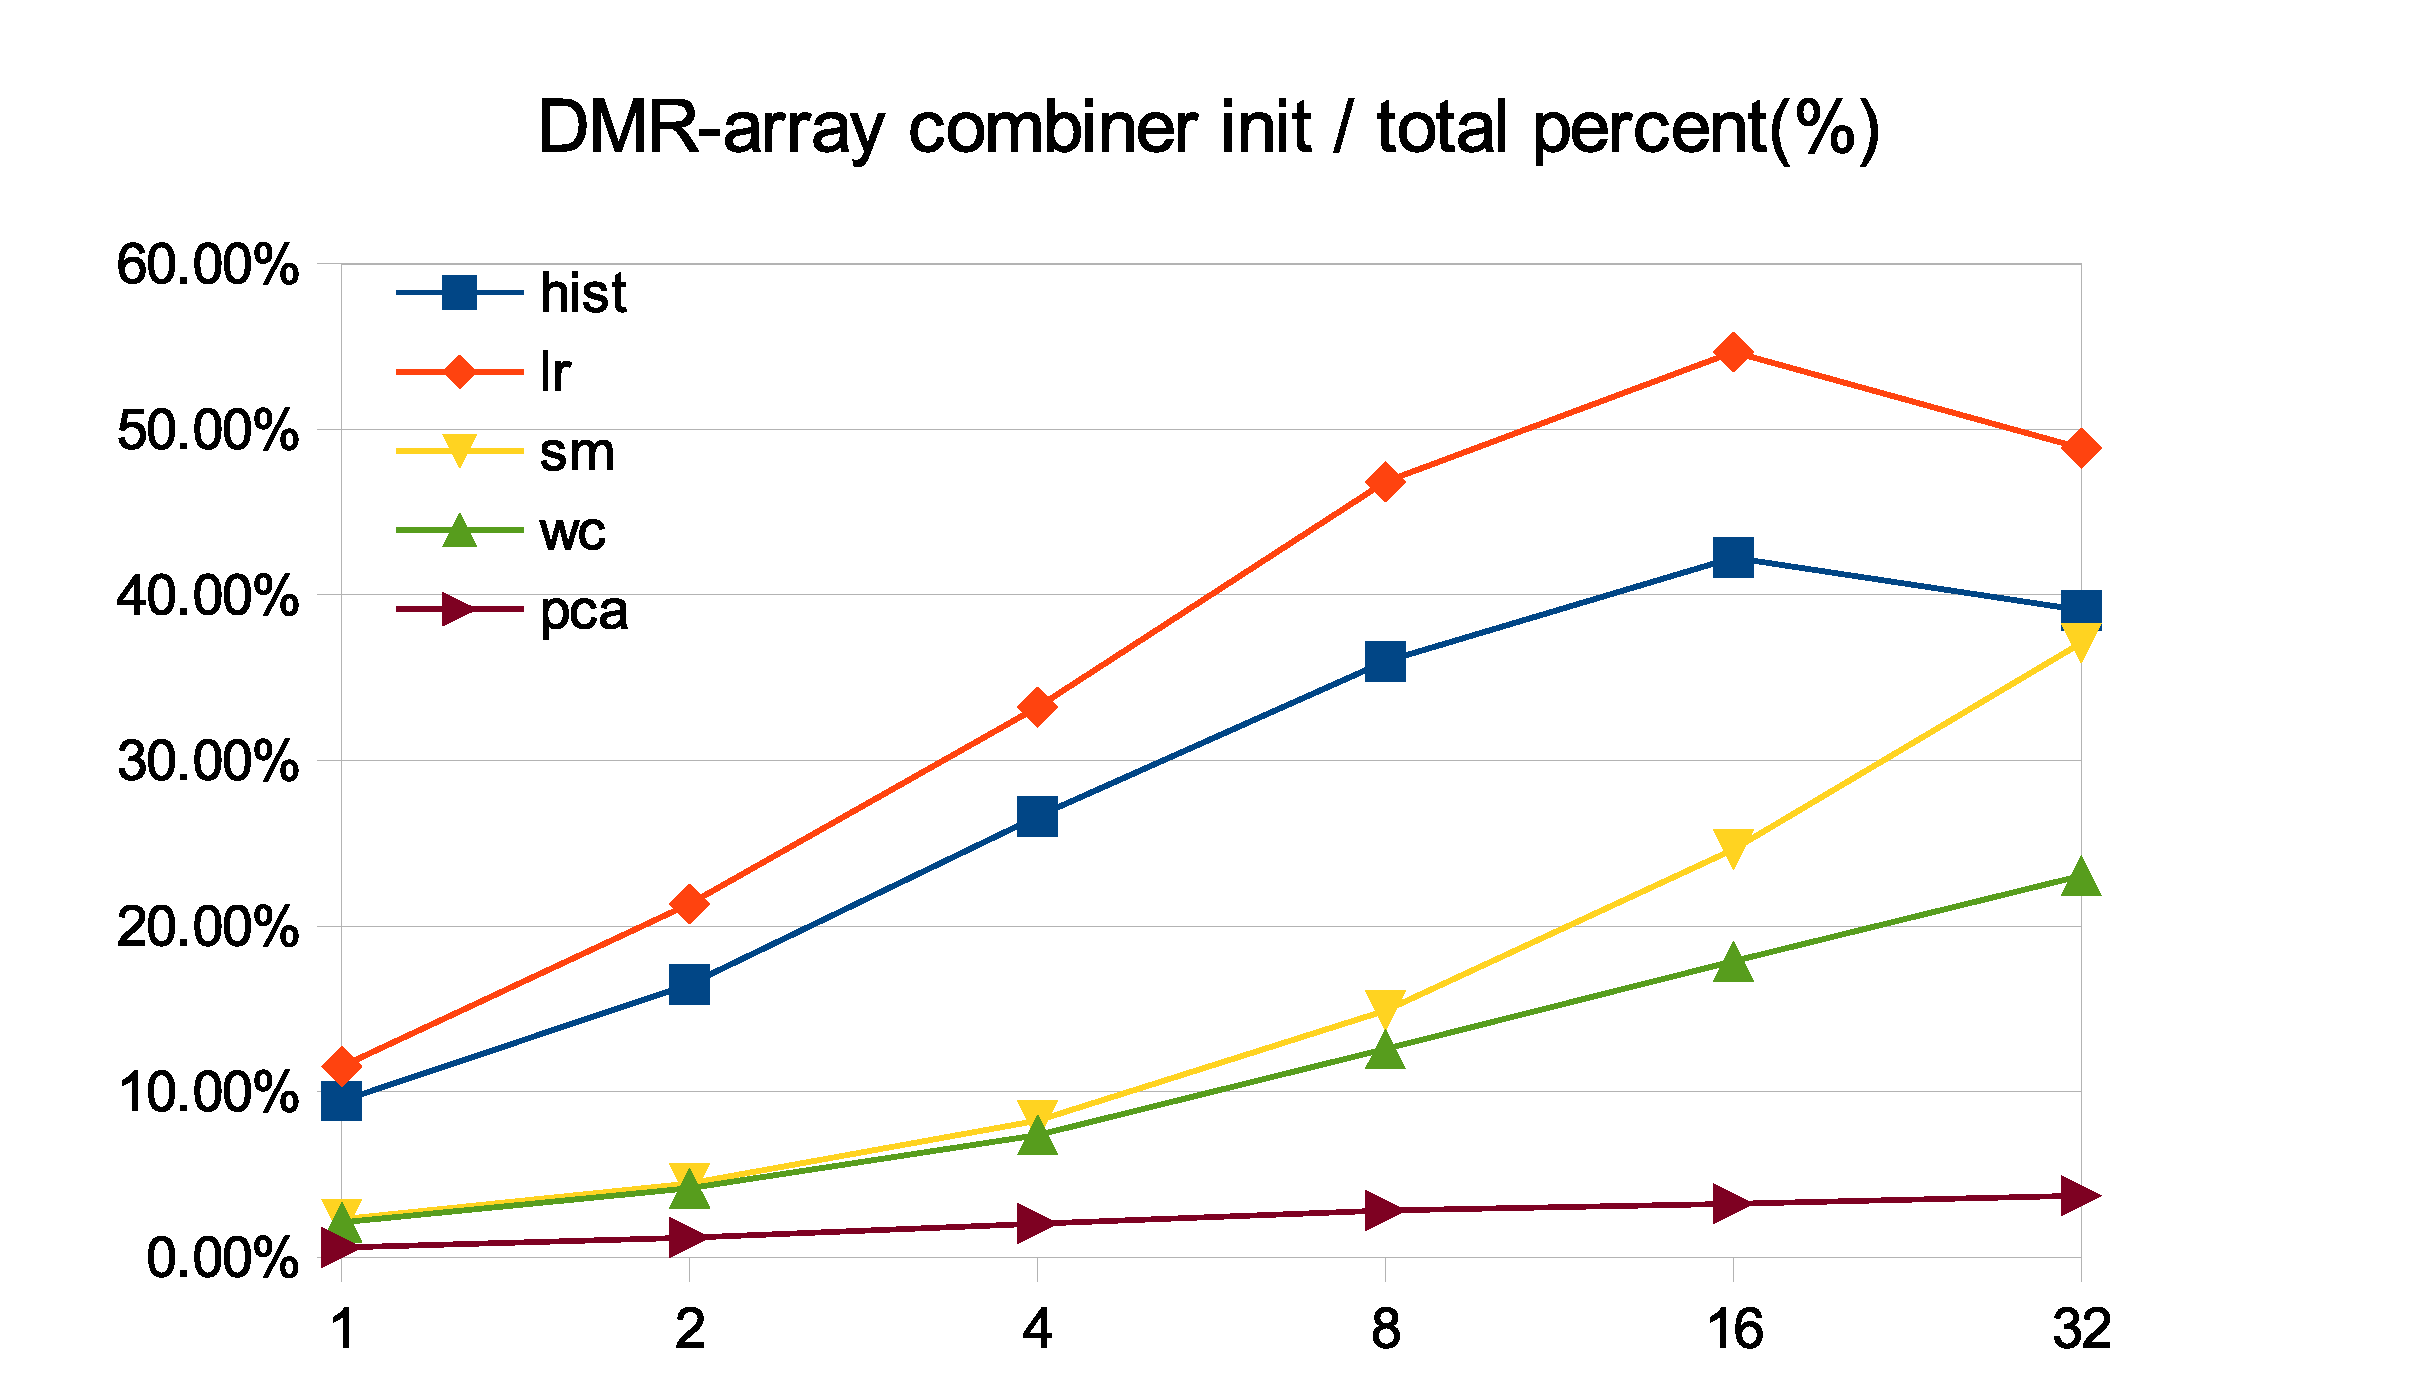
\includegraphics[width=0.4\textwidth]{eps/dmr_init.eps}
   \label{fig:dmr:time:jemalloc}
  }
  \caption{Initialize time of SMR and Phoenix}
   \label{fig:time}
\end{figure}

\redt{\myds initialization time is uesd to create threads, channel.}
%\myds的大部分时间用于了thread的创建,channel的分配,因此它的开销远大于Phoenix初始化的开销





\section{Related Work}
%两个方面:(1)面向多核的mapreduce的研究:Phoenix, mutis, MRPhi (2)linux scalability的问题
\label{sec:rel}
%在写这一部分的时候,需要将全部收集的论文重新看一边,并修改论文中的设计部分,最后,写好abstract, introduction, related work.

Our work is related to the research in programming models for
data-parallel applications, nested data parallelism and multicore re-
lated research. We briefly discuss the most related work in turn.
\subsection{MapReduce programming model}
MapReduce is a popular distributed framework
for massive-scale parallel data analysis.
There are many existing implementation of MapReduce 
which adopt on the basic architecture and 
programming model of originally Google's MapReduce, 
such as Hadoop\cite{}, Dryad\cite{isard2007dryad}.

The Phoenix MapReduce libray
is the most relevant work to \myds. 
Phoenix demostrate that MapReduce is a promising parallel programming
models in muliticore and multiprocess systems.
It creates a thread pool by Pthreads
and can schedule tasks dynamically to support itrative applications.
\myds differs from Phoenix mainly on that 
Phoenix need barrier between iterative MapReduce,
while \myds brokes barrier to speed up computing.

%虽然我们没有与mites, Tilt-MapReduce进行对比,但通过我们的研究,只要这些库使用pthread进行编程,那么就会存在scalability较差的问题。
Tilt-MapReduce\cite{chen2010tiled}
This paper argued that the environmental differences between
clusters and multicore open new design spaces and optimization
opportunities to improve performance of MapReduce on multicore.
Based on the observation, this paper proposed Tiled-MapReduce,
that uses the “tiling strategy” to partition a large MapReduce job
into a number of small sub-jobs and handles the sub-jobs itera-
tively. This paper also explored several optimizations otherwise im-
possible for MapReduce, to improve the memory, cache and CPU
efficiency.

Although, we don't compare \myds with mites, Tilt-MapReduce,
our research shows that if the MapReduce library implemented by Pthreads, there will be problem of scalability.

Metis\cite{mao2010metis},The paper’s main insight is that the organiza-
tion of the intermediate values produced by Map invocations and consumed by Reduce invocations is central
to achieving good performance on multicore processors.
Metis stores these intermediate values using an efficient
data structure consisting of a hash table per Map thread
with a b+tree in each hash entry. As a result, Metis can
achieve better performance than Phoenix on MapReduce
applications that interact with the library frequently (e.g.,
applications with many keys).

MRPhi\cite{} is a multicore mapreduce.

\subsection{Scalability of multicore}
A multicore operating system, named Corey\cite{boyd2008corey}, proposes three
new abstractions (address ranges, shares and kernel cores), to scale
a MapReduce application (i.e., Word Revert Index) running on Corey.
The work in Corey is orthogonal to Ostrich. The abstractions in
Corey, if available in commodity OSes, could further improve the
efficiency of Ostrich due to the reduced time spent in the OS kernel.
	
An Analysis of Linux Scalability to Many Cores \cite{Boyd2010An},
This paper analyzes the scaling behavior of a traditional
operating system (Linux 2.6.35-rc5) on a 48-core com-
puter with a set of applications that are designed for par-
allel execution and use kernel services. We find that we
can remove most kernel bottlenecks that the applications
stress by modifying the applications or kernel slightly.

RadixVM\cite{Clements2013RadixVM}RadixVM, a new virtual memory design
that allows VM-intensive multithreaded applications to scale
with the number of cores.



\section{Conclusions And Furture Work}
\label{sec:concl}
We have presented \myds,
a scalable iterative MapReduce model, 
to support efficient iterative processing.

Our evaluation further shows the scalability and reliablity of \myds
for iterative processing.
As to poor performance on multicast across processors,
our future work will provide NUMA-aware scalable iterative processing.
And supporting online-MapReduce.
\iffalse
\section*{Acknowledgment} 
{\small
This work was supported in part by 
the National High Technology Research and Development Program
of China (863 Program) grant (No.2012AA010901),
and the National Natural Science Foundation of China Grant (No.61170018).}
\fi


\begin{small}
%\begin{footnotesize}
\bibliography{os,pa,my}
\bibliographystyle{abbrvnat}
%\bibliographystyle{plain}
%\end{footnotesize}
\end{small}

\end{document}
